\documentclass[twocolumn, 10pt]{article}

\usepackage{amsmath}
\usepackage{graphicx}
\graphicspath{ {./images/} }

\title{2XC3 - Lab 1 Report}
\author{Oleg Glotov\\ L03, 400174037\\ glotovo@mcmaster.ca \and Banjo Maccio\\ Dogtown Hamilton\\ goodboy@mcmaster.ca}


\begin{document}
\maketitle
\section{Git Setup}\label{sec:git}
The group began by setting up out github accounts and the repository. The visibility was set to private to comply with McMaster's code of conduct.

\begin{figure}[h]
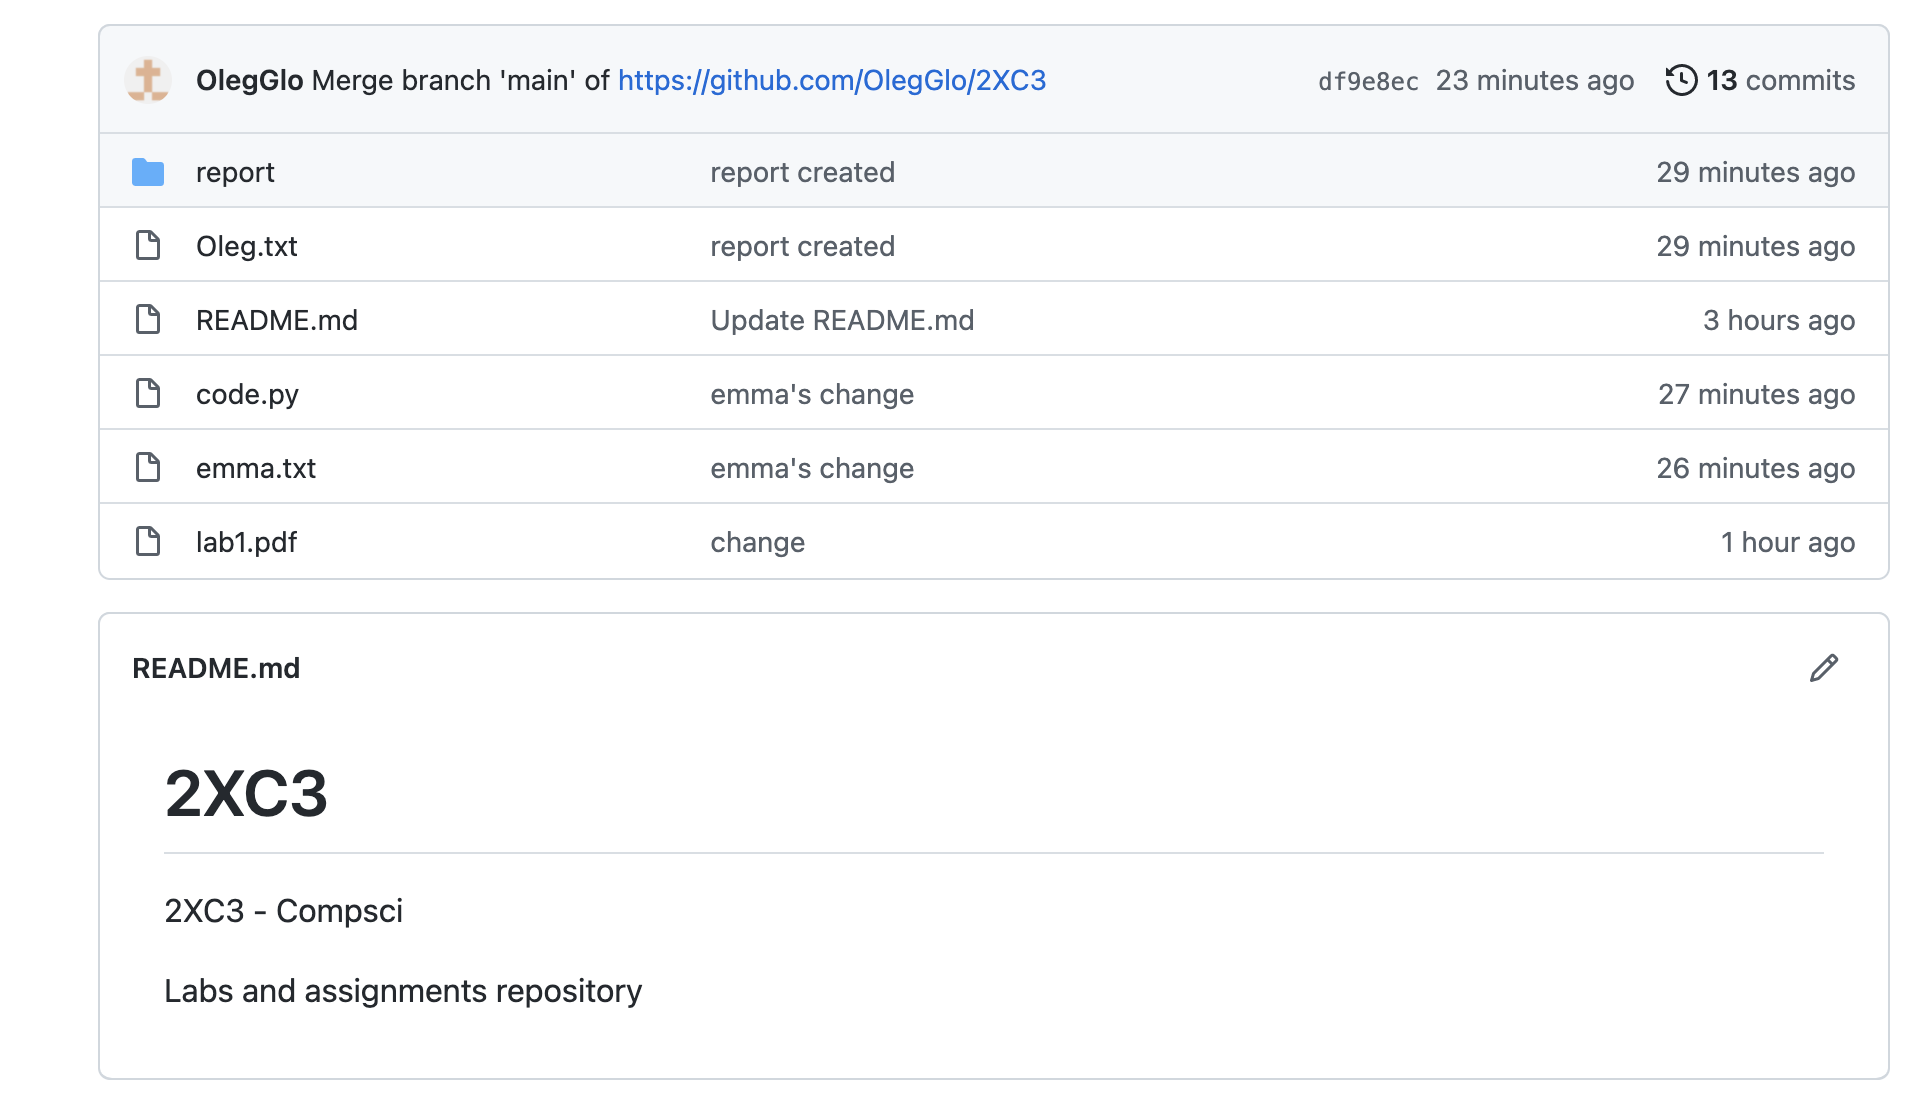
\includegraphics[width=\linewidth]{img1}
\end{figure}

\footnotesize
\begin{verbatim}
def are_valid_groups(groups, studentNum):

    length = len(studentNum)
    count = 0
    
    for group in groups:
        count = 0
        for students in studentNum:
            if (group.count(students) == 0):
                break
            if (group.count(students) == 1):
                count += 1
        
        if count == length:
            return True
        
    return False

print(are_valid_groups(groups, studentNum))
\end{verbatim}
\normalsize

\begin{center}
\begin{table}[!h]
\begin{tabular}{|l|l|l|}
\hline
x     & y          & z    \\ \hline
1     & 22         & 3    \\ \hline
$y+4$ & $k\cdot x$ & text \\ \hline
\end{tabular}
\end{table}
\end{center}

\section{First Lesson}
\section{Second Lesson}
\section{Conclusion}
\end{document}

